
%----------------------------------------------------------------------------------------%
% START LaTeX preamble

% define document type, font and paper size
\documentclass[11pt,a4paper]{article}

%----------------------------------------------------------------------------------------%
% IMPORT LaTeX packages

\usepackage{inputenc}
\usepackage[ngerman, english]{babel}
\usepackage{csquotes}
\usepackage{amsmath}
\usepackage{amssymb}
\usepackage{amsfonts}
\usepackage{media9}
\usepackage{graphicx}
\usepackage{wrapfig}
\usepackage[margin=1.25in]{geometry}
\usepackage{pdfpages}
\usepackage{listings}
\usepackage{setspace}
\usepackage{systeme}
\usepackage{mdframed}
\usepackage{mmacells}

\newcommand{\mathsym}[1]{{}}
\newcommand{\unicode}[1]{{}}

%----------------------------------------------------------------------------------------%
% IMPORT LaTeX packages to manange bibliography

% MLA, APA, or IEEE? - https://www.overleaf.com/learn/latex/Biblatex_citation_styles
\usepackage[style=apa, backend=biber]{biblatex}
\addbibresource{bibliography.bib}

%----------------------------------------------------------------------------------------%
% DEFINE header values

% define the cover page values
\title
{
    Mathematica Problem Sheet 01
}
\author
{    
    Antonio Osamu Katagiri Tanaka (A01212611) \\
    \\
    Instructor: Ph.D Daniel L{\' o}pez Aguayo
}
\date{\today}

%----------------------------------------------------------------------------------------%
% USER-DEFINED commands

% Keywords command
\providecommand{\keywords}[1]
{
    \\
    \\
    \small
    \textbf{\textit{Keywords:}} #1
}

%----------------------------------------------------------------------------------------%

\begin{document}
\setlength\parindent{0pt} % Set noindent for entire file

%----------------------------------------------------------------------------------------%
% CREATE the 1st page (cover page)

\maketitle

%----------------------------------------------------------------------------------------%
% DEFINE the abstract text & keywords

%\begin{abstract}
%    \emph
%    {
%        Lorem ipsum dolor sit amet, consectetur adipiscing elit, sed do eiusmod tempor incididunt ut labore et dolore magna aliqua. Ut enim ad minim veniam, quis nostrud exercitation ullamco laboris nisi ut aliquip ex ea commodo consequat. Duis aute irure dolor in reprehenderit in voluptate velit esse cillum dolore eu fugiat nulla pariatur. Excepteur sint occaecat cupidatat non proident, sunt in culpa qui officia deserunt mollit anim id est laborum.
%    }
%    \keywords{Lorem, ipsum, dolor, sit, amet}
%\end{abstract}
\clearpage

%----------------------------------------------------------------------------------------%
% CREATE a table of contents in a new page

%\tableofcontents
%\clearpage

%----------------------------------------------------------------------------------------%
% CREATE a list of figures and a list of tables in a new page

%\listoffigures
%\listoftables
%\clearpage

%----------------------------------------------------------------------------------------%
% DOCUMENT body starts here

%----------------------------------------------------------------------------------------%
%Append the HW's exercises
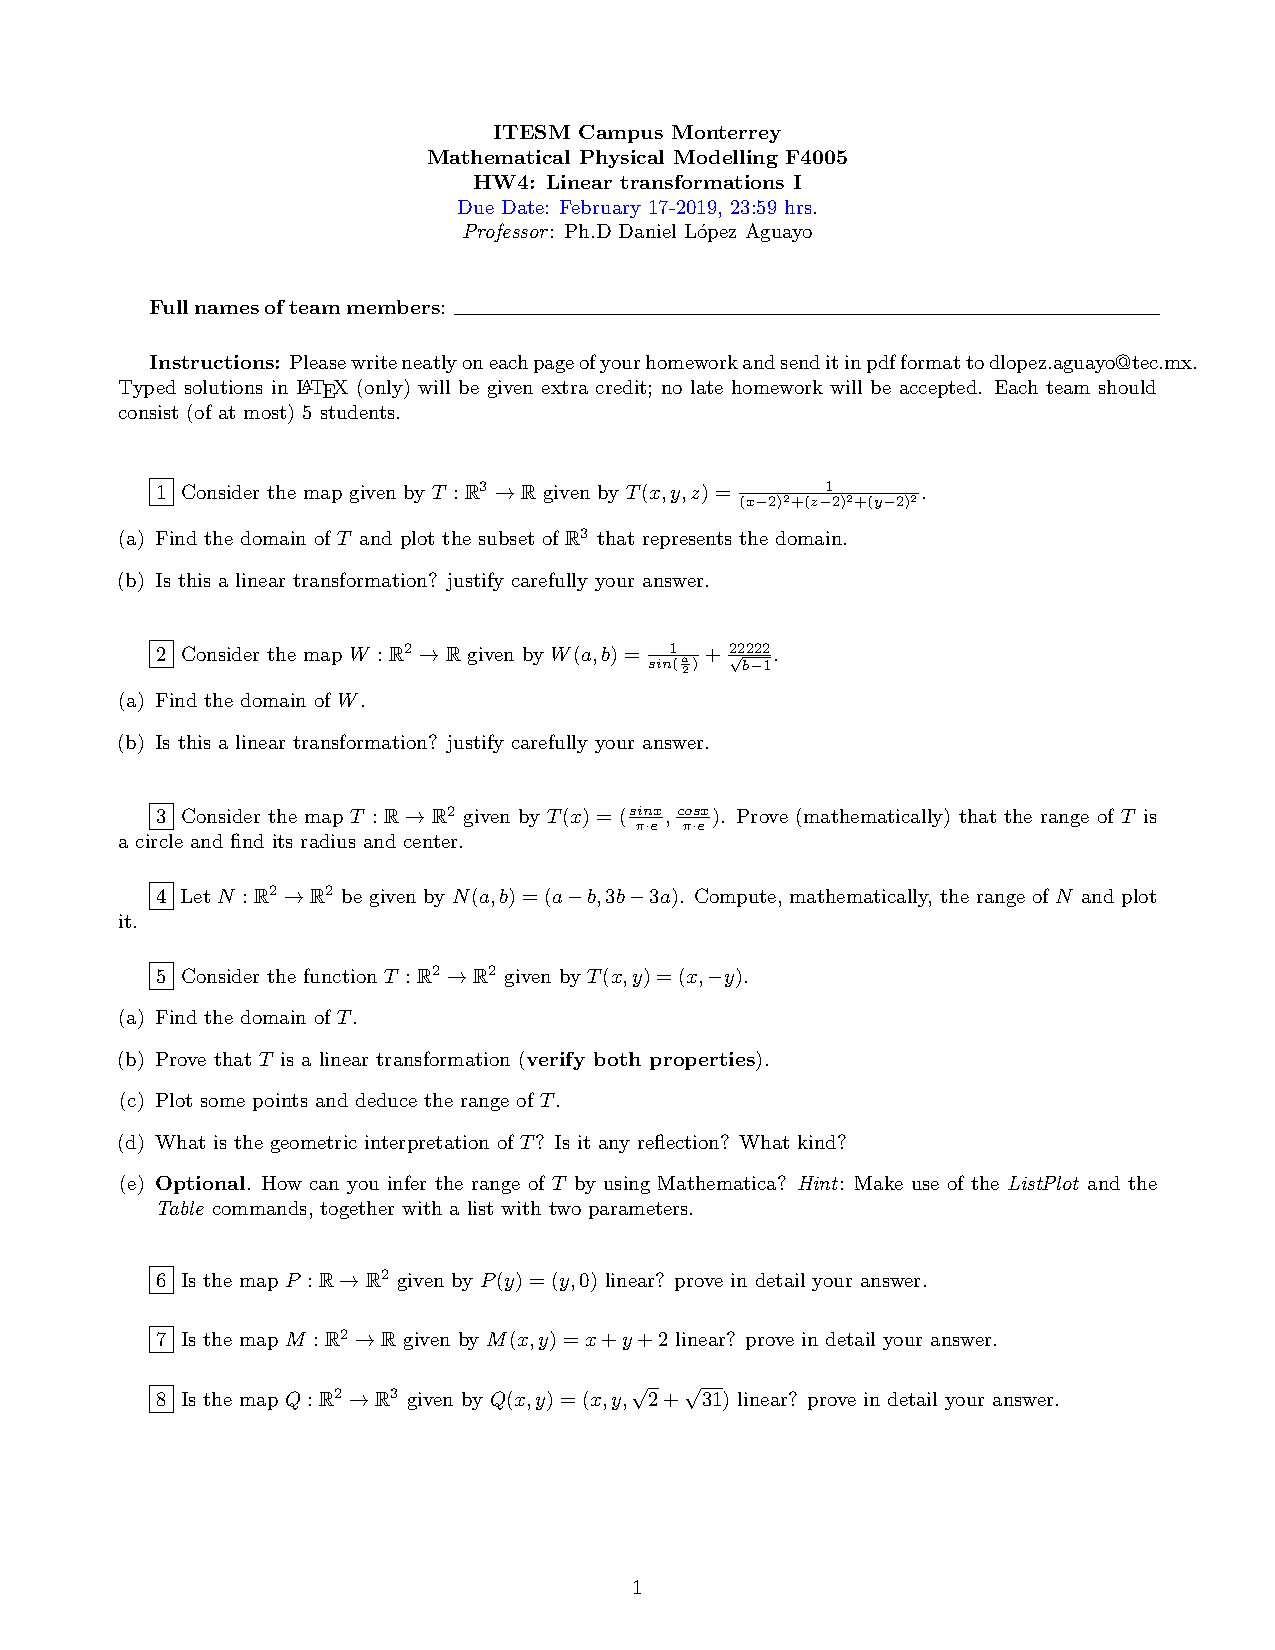
\includepdf[page=-]{HW4}

%----------------------------------------------------------------------------------------%
\section{Answer to Problem I}\label{sec:P01}

\subsection{}
\begin{mmaCell}{Print}
T:\mmaSup{\(\pmb{\mathbb{R}}\)}{3}\(\pmb{\rightarrow}\)\(\pmb{\mathbb{R}}\) given by T(x,y,z)=\mmaFrac{1}{\mmaSup{(x-2)}{2}+\mmaSup{(z-12)}{2}+\mmaSup{(x-2)}{2}}
\mmaSub{D}{(T)}=\mmaSup{\(\pmb{\mathbb{R}}\)}{3}
\end{mmaCell}

\begin{mmaCell}[moredefined={T, contourLimits, membershipConditions, domain, myPlot}]{Input}
T=\mmaFrac{1}{(x-2)^2+(z-12)^2+(y-2)^2};
contourLimits=100;
membershipConditions=FunctionDomain[T,\{x,y,z\}];
domain=ImplicitRegion[membershipConditions,\{x,y,z\}];

Print["Domain:"];
RegionMember[domain,\{x,y,z\}]
myPlot=RegionPlot3D[domain,Axes\(\pmb{\to}\)True]
Export["./media/problem1aDomain.png",myPlot];

Print["Domain subset Plot:"];
myPlot=Plot3D[T,\{x,y,z\}\(\pmb{\in}\)domain,Axes\(\pmb{\to}\)True]
Export["./media/problem1aDomainSubset1.png",myPlot];
myPlot=DensityPlot3D[T,\{x,y,z\}\(\pmb{\in}\)domain,Axes\(\pmb{\to}\)True]
Export["./media/problem1aDomainSubset2.png",myPlot];
myPlot=ContourPlot3D[T,\{x,y,z\}\(\pmb{\in}\)domain,Axes\(\pmb{\to}\)True]
Export["./media/problem1aDomainSubset3.png",myPlot];
\end{mmaCell}

\begin{mmaCell}{Print}
Domain:
\end{mmaCell}

\begin{mdframed}
\begin{mmaCell}[]{Output}
(x|y|z)\(\in\mmaSup{R}\)&&-4 x+\mmaSup{x}{2}-4y+\mmaSup{y}{2}-24z+\mmaSup{z}{2}\(\neq\)-152
\end{mmaCell}
\end{mdframed}

\begin{mmaCell}[]{Output}

\end{mmaCell}
\begin{figure}[!h]
\centering
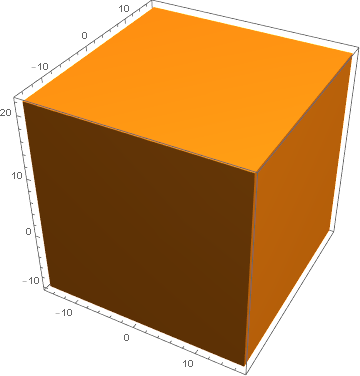
\includegraphics[width=0.45\textwidth]{./media/problem1aDomain.png}
\caption{Domain of T.\label{figure_ambush}}
\end{figure}

\begin{mmaCell}{Print}
Domain subset Plot:
\end{mmaCell}

\begin{mmaCell}[]{Output}
Plot3D[T,\{x,y,z\}\(\in\)domain,Axes\(\to\)True]
\end{mmaCell}

\begin{mmaCell}[]{Output}

\end{mmaCell}
\begin{figure}[!h]
\begin{mdframed}
\centering
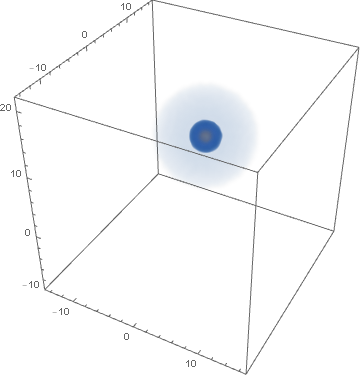
\includegraphics[width=0.45\textwidth]{./media/problem1aDomainSubset2.png}
\end{mdframed}
\caption{Subset that represents the domain.\label{figure_ambush}}
\end{figure}

\begin{mmaCell}[]{Output}
ContourPlot3D[T,\{x,y,z\}\(\in\)domain,Axes\(\to\)True]
\end{mmaCell}

\subsection{}
\begin{mmaCell}[moredefined={T}]{Print}
a) Check T preserves sums

let u=(a,b,c), v=(d,e,f) be elements of \mmaSup{\mmaUnd{\(\pmb{\mathbb{R}}\)}}{3}
T(u+v)=T((a,b,c)+(d,e,f))
      =T(a+d,b+e,c+f)
      =\mmaFrac{1}{\mmaSup{(a+d-2)}{2}+\mmaSup{(c+f-12)}{2}+\mmaSup{(b+e-2)}{2}}

T(u)+T(v)=T(a,b,c)+T(d,e,f)
         =\mmaFrac{1}{\mmaSup{(a-2)}{2}+\mmaSup{(c-12)}{2}+\mmaSup{(b-2)}{2}}+\mmaFrac{1}{\mmaSup{(d-2)}{2}+\mmaSup{(f-12)}{2}+\mmaSup{(e-2)}{2}}

T is NOT a linear transformation since it does not preserve sums.

b) Check T preserves scalars
   no need to check ...
\end{mmaCell}

\clearpage

%----------------------------------------------------------------------------------------%
\section{Answer to Problem II}\label{sec:P02}

\subsection{}
\begin{mmaCell}{Print}
T:\mmaSup{R}{2}\(\pmb{\rightarrow}\)R given by W(a,b)=\mmaFrac{1}{Sin[\mmaFrac{a}{2}]+\mmaFrac{22222}{\mmaSqrt{b-1}}}
\mmaSub{D}{(T)}=\mmaSup{R}{2}
\end{mmaCell}

\begin{mmaCell}[moredefined={W, contourLimits, membershipConditions, domain, domainRegion, myPlot}]{Input}
W=\mmaFrac{1}{Sin[\mmaFrac{a}{2}]+\mmaFrac{22222}{\mmaSqrt{b-1}}};
contourLimits=100;
membershipConditions=FunctionDomain[W,\{a,b\}];
domain=ImplicitRegion[membershipConditions,\{a,b\}];

Print["Domain:"];
domainRegion=RegionMember[domain,\{a,b\}]
myPlot=RegionPlot[domainRegion,\{\mmaFnc{a},0,15\},\{\mmaFnc{b},0,15\},Axes\(\pmb{\to}\)True]
Export["./media/problem2aDomain.png",myPlot];
\end{mmaCell}

\begin{mmaCell}{Print}
Domain:
\end{mmaCell}

\begin{mdframed}
\begin{mmaCell}[]{Output}
(a|b)\(\in\mathbb{R}\)&&b>1&&\mmaFrac{22222}{\mmaSqrt{-1+b}}+Sin[\mmaFrac{a}{2}]\(\neq\)0
\end{mmaCell}
\end{mdframed}

\begin{mmaCell}[]{Output}

\end{mmaCell}
\begin{figure}[!h]
\centering
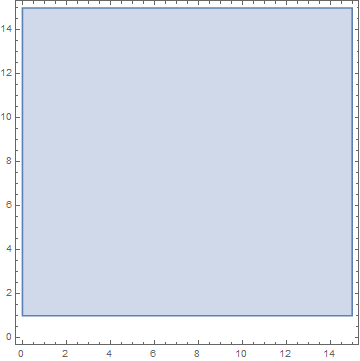
\includegraphics[width=0.45\textwidth]{./media/problem2aDomain.png}
\caption{Subset that represents the domain.\label{figure_ambush}}
\end{figure}

\clearpage

\subsection{}
\begin{mmaCell}[moredefined={T}]{Print}
a) Check T preserves sums

let u=(a,b), v=(d,e) be elements of \mmaSup{\mmaUnd{\(\pmb{\mathbb{R}}\)}}{2}
T(u+v)=T((a,b)+(d,e))
      =T(a+d,b+e)
      =\mmaFrac{1}{Sin[\mmaFrac{a+d}{2}]+\mmaFrac{22222}{\mmaSqrt{b+e-1}}}

T(u)+T(v)=T(a,b)+T(d,e)
         =\mmaFrac{1}{Sin[\mmaFrac{a}{2}]+\mmaFrac{22222}{\mmaSqrt{b-1}}}+\mmaFrac{1}{Sin[\mmaFrac{d}{2}]+\mmaFrac{22222}{\mmaSqrt{e-1}}}

\boxed{T is NOT a linear transformation since it does not preserve sums.}

b) Check T preserves scalars
no need to check ...
\end{mmaCell}

\clearpage

%----------------------------------------------------------------------------------------%
\section{Answer to Problem III}\label{sec:P03}

\subsection{}
\begin{mmaCell}{Print}
A circle can be described as the set of points (x,y) that satisfy
\mmaSup{x}{2}+\mmaSup{y}{2}=\mmaSup{r}{2}. Hence, if x=\mmaFrac{Sin[x]}{\(\pmb{\pi}\)e} and y=\mmaFrac{Cos[x]}{\(\pmb{\pi}\)e} then
\mmaSup{x}{2}+\mmaSup{y}{2}=\mmaSup{(\mmaFrac{Sin[x]}{\(\pmb{\pi}\)e})}{2}+\mmaSup{(\mmaFrac{Cos[x]}{\(\pmb{\pi}\)e})}{2}=\mmaSup{r}{2} ; where r is the radius.
\end{mmaCell}

\subsection{}
\begin{mmaCell}{Input}
radius=FullSimplify[\mmaSqrt{\mmaSup{(\mmaFrac{Sin[x]}{\mmaDef{\(\pmb{\pi}\)} \mmaDef{e}})}{2}+\mmaSup{(\mmaFrac{Cos[x]}{\mmaDef{\(\pmb{\pi}\)}\mmaDef{e}})}{2}}];
radius
N[%]
\end{mmaCell}

\begin{mdframed}
\begin{mmaCell}{Print}
The circle equation is in the format \mmaSup{(x--h)}{2}+\mmaSup{(y--k)}{2}=\mmaSup{r}{2}, with the
center being at the point (h,k) and the radius being "r". Since
h & k are equal to zero, then the center is at the origin.
\end{mmaCell}
\end{mdframed}

\begin{mdframed}
\begin{mmaCell}{Output}
\mmaFrac{1}{e \(\pi\)}
\end{mmaCell}

\begin{mmaCell}{Output}
0.1171
\end{mmaCell}
\end{mdframed}

\subsection{}
\begin{mmaCell}[moredefined={T, contourLimits, membershipConditions, domain, points, plots, frames, myPlot},morefunctionlocal={n}]{Input}
ClearAll["Global`*"];
T=\{\mmaFrac{Sin[x]}{\mmaDef{\(\pmb{\pi}\)}*\mmaDef{e}},\mmaFrac{Cos[x]}{\mmaDef{\(\pmb{\pi}\)}*\mmaDef{e}}\};

contourLimits=100;
membershipConditions=FunctionDomain[T,\{x\}];
domain=ImplicitRegion[membershipConditions,\{x\}];

Print["Range:"];
points=Table[\{\mmaFrac{Sin[\mmaFnc{x}]}{\mmaDef{\(\pmb{\pi}\)}*\mmaDef{e}},\mmaFrac{Cos[\mmaFnc{x}]}{\mmaDef{\(\pmb{\pi}\)}*\mmaDef{e}}\},\{\mmaFnc{x},-150,150\}];
ListPlot[points]
plots = Table[
    Show[Graphics[Point[points[[n]]]],
    PlotRange \(\pmb{\to}\)\{\{-0.12,0.12\},\{-0.12,0.12\}\},
    Axes\(\pmb{\to}\)Automatic],
    \{n,Length[points]\}
];
frames=FoldList[Show,plots];
myPlot=ListAnimate[frames,AnimationRate\(\pmb{\to}\)60]
Export["./media/problem3aRange.swf",myPlot];
\end{mmaCell}

\begin{mmaCell}{Output}
Range:
\end{mmaCell}
\begin{figure}[!h]
\centering
\includemedia[
  width=0.50\textwidth,
  totalheight=0.60\textwidth,
  activate=pageopen,
]{\fbox{problem3aRange.swf}}{./media/problem3aRange.swf}
\caption{Range of T.\label{figure_ambush}}
\end{figure}

\clearpage

%----------------------------------------------------------------------------------------%
\section{Answer to Problem IV}\label{sec:P04}



\clearpage

%----------------------------------------------------------------------------------------%
\section{Answer to Problem V}\label{sec:P05}



\clearpage

%----------------------------------------------------------------------------------------%
\section{Answer to Problem VI}\label{sec:P06}



\clearpage

%----------------------------------------------------------------------------------------%
\section{Answer to Problem VII}\label{sec:P07}



\clearpage

%----------------------------------------------------------------------------------------%
\section{Answer to Problem VIII}\label{sec:P08}



\clearpage

%----------------------------------------------------------------------------------------%
\section{Answer to Problem IX}\label{sec:P09}



\clearpage

%----------------------------------------------------------------------------------------%
\section{Answer to Problem X}\label{sec:P10}



\clearpage

%----------------------------------------------------------------------------------------%
\section{Answer to Problem XI}\label{sec:P11}



\clearpage

%----------------------------------------------------------------------------------------%
\section{Answer to Problem XII}\label{sec:P12}



\clearpage

%----------------------------------------------------------------------------------------%
% PRINT bibliography/references in a new page

%\clearpage
\printbibliography

%----------------------------------------------------------------------------------------%

\end{document}

%----------------------------------------------------------------------------------------%
